\chapter{Lec 04 - PAC, Generalization and SRM}
\section{Hoeffding's Inequality}
Let's start with an example. Consider a bin full of red and green marbles.
\begin{center}
    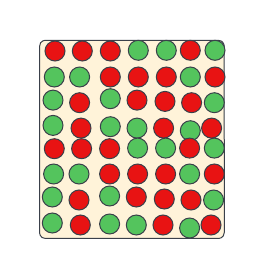
\includegraphics{images/Marbles Bin.png}
\end{center}
We denote:
\begin{itemize}
    \item $P(red) = \pi$ the probability to draw a red marble (unknown)
    \item $P(green) = 1 - \pi$ the probability to draw a green marble (unknown)
\end{itemize}
Then we draw $N$ marbles (the \textit{sample}) from the bin, \textbf{independently}\footnote{the draw of one marble doesn't influence the draw of the next one}, and we set $\sigma$ as the fraction of red marbles in the sample. So $\pi$ represent the proportion of red marbles in the \textbf{bin}, while sigma represent the proportion of red marbles in the \textbf{sample}. So the question is, does $\sigma$ say anything about $\pi$?

Consider the following formula:
\begin{center}
    \[P(|\sigma - \pi| > \epsilon) \leq 2e^{-2\epsilon^{2}N}\]
\end{center}
It's called \textbf{Hoeffding's Inequality} and it means that in a large sample (large $N$), the value of $\sigma$ is likely close to $\pi$ (within $\epsilon$).
\begin{itemize}
    \item $|\sigma - \pi| > \epsilon$ is called \textit{bad event} because when the absolute value of the difference between $\sigma$ an $\pi$ is greater than $\epsilon$, it means that $\sigma$ an $\pi$ are not so similar. This event depends on the \textit{tolerance} value $\epsilon$ that we choose.
    
    \item $2e^{-2\epsilon^{2}N}$ is a negative exponential curve.
    \begin{flushleft}
        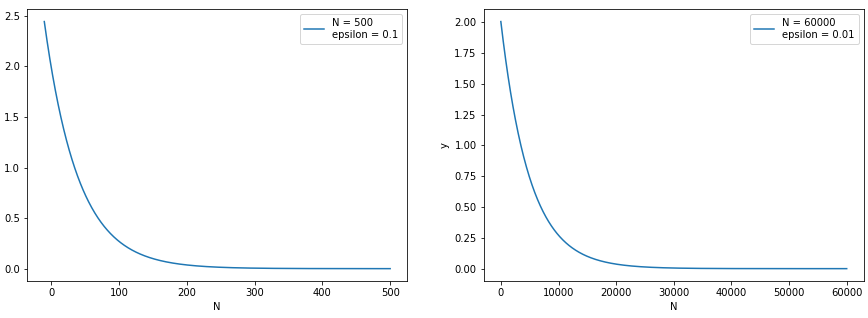
\includegraphics[scale = 0.45]{images/exp.png}
    \end{flushleft}
    As you can see from the graphs above, the curve decreases as N increases. So with larger samples, the \textit{bad event} will occur with a lower probability. Furthermore, if we set a stricter tolerance value (e.g $\epsilon$ = 0.01) the curve decreases more slowly.
\end{itemize}
For example, if we set $\epsilon$ = 0.1, $P(|\sigma - \pi| > \epsilon)$ is the probability of having a discrepancy between $\sigma$ and $\pi$ greater than 10\%; this probability, for $N$ = 200, is $\leq 0.03663127777746833$. So $\sigma = \pi$ is \textbf{P.A.C} (Probably Approximately Correct).

\section{Connection to Learning}
\begin{itemize}
    \item The target function $f: X \rightarrow Y$ is unknown
    \item The bin is the input space $X$ which contains all possible inputs for a model.
    \item The sample $N$ is the training set.
    
    \item The training set is composed by a set of pairs $\{(\textbf{x}_{1},y_{1}),...,(\textbf{x}_{n},y_{n})\}$ where $y_{i} = f(\textbf{x}_{i})$. Once we have fixed an hypothesis $h: X \rightarrow Y$ (chosen from the hypothesis space), we can "color" each example in $N$ as follows:
    \begin{itemize}
        \item green if $h(\textbf{x}) = f(\textbf{x})$
        \item red if $h(\textbf{x}) \neq f(\textbf{x})$
    \end{itemize}
    \begin{center}
        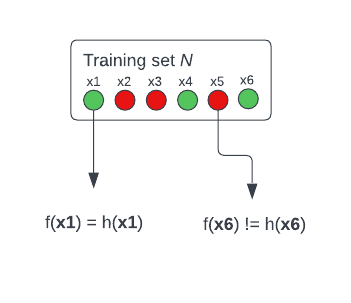
\includegraphics{images/Training set.png}
    \end{center}
\end{itemize}
Now we can say that $\sigma$ is the \textbf{empirical error}, while $\pi$ is the \textbf{ideal error} (for this $h$) and following the previous example we can observe that $\sigma$ tends to be close to $\pi$. If we have a small error $\sigma$ it's more and more probable that $h$ is a good approximation of the target function \textbf{in general} as $N$ increases. So this process \textbf{verifies} how good the approximation $h$ of $f$ is, but it has nothing to do with learning process, because $\pi$ and $\sigma$ depend on which $h$ we choose. How do we choose $h$?
\subsection{Learning}
First of all, let's change the notation:
\begin{itemize}
    \item empirical error on training data $\sigma \rightarrow E_{i}(h)$
    \item ideal error $\pi \rightarrow E_{o}(h)$
    \item $P(|E_{i}(h) - E_{o}(h)| > \epsilon) \leq 2e^{-2\epsilon^{2}N}$. The bound depends on $h$
\end{itemize}
The hypothesis space $H \equiv \{h_{1}, h_{2},...,h_{m}\}$ it's composed by many different hypotheses $h_{1},..,h_{m}$ and each of them has an empirical error $E_{i}(h_{i})$ and an ideal error $E_{o}(h_{i})$. Learning algorithms search in the hypothesis space (following some criterion) and select an hypothesis $h_{i}$ that minimizes $E_{o}(h_{i})$. However, the Hoeffding's Inequality can't be used for learning because in Supervised Learning we have to choose among several hypotheses. If we consider a worst case analysis, where all the bad events over the hypothesis space are \textbf{disjointed}, we have to bound the probability of interest in the following way:
\[P[|E_{i}(h_{i}) - E_{o}(h_{i})| > \epsilon] \leq \sum_{m=1}^{M}P[|E_{i}(h_{m}) - E_{o}(h_{m})| > \epsilon] \leq 2Me^{-2\epsilon^{2}N}\] where $M$ is the number of hypotheses (can also be infinite). \newline

The formula above says that since $h_{i}$ can be any of all $h_{1},..,h_{m}$ hypotheses in the hypothesis space, the bad event $|E_{i}(h_{i}) - E_{o}(h_{i})| > \epsilon$ can happen for $h_{1}$ \textbf{or} for $h_{2}$ \textbf{or} for $h_{3}$ \textbf{or} ... for $h_{m}$. So, since we are assuming that all bad events are disjointed ($P(A \cup B) = P(A) + P(B)$), $P[|E_{i}(h_{i}) - E_{o}(h_{i})| > \epsilon]$ must be bounded by $\sum_{m=1}^{M}P[|E_{i}(h_{m}) - E_{o}(h_{m})| > \epsilon]$. Note that for very big M the resulting bound is $>>1$, so it's useless.\newline

Just to recap a little bit:
\begin{itemize}
    \item \textbf{Testing:} Hoeffding's Inequality can help us to verify if a \textbf{fixed} hypothesis $h$ is a good approximation of the target function $f$ over a sample $N$.
    \item \textbf{Training:} Hoeffding's Inequality is not so useful for learning process since we have to choose among several hypotheses.
\end{itemize}

Fortunately, bad events are not always disjointed but they are overlapped.
\begin{center}
    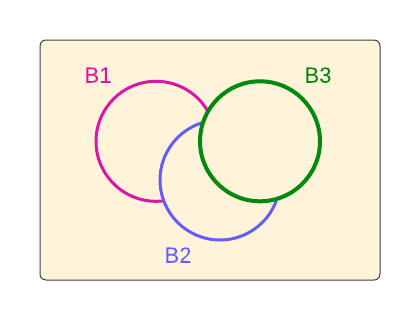
\includegraphics{images/Overlapped Sets.png}
\end{center}
So $M$ can be replaced by the \textbf{growth function} $m_{H}(N) \leq 2^{N}$ which is related to the complexity of the hypothesis space. When the hypothesis space has a low complexity bad events overlap a lot ($m_{H}(N) << 2^{N}$), when it's very complex they tend to be disjointed. So if $m_{H}(N)$ is \textbf{polynomial} with respect to $N$, the upper bound $2Me^{-2\epsilon^{2}N}$ tends to 0 as $N$ increases. How can i compute the complexity of the hypothesis space ?
\subsection{VC-Dimension}
\begin{center}
    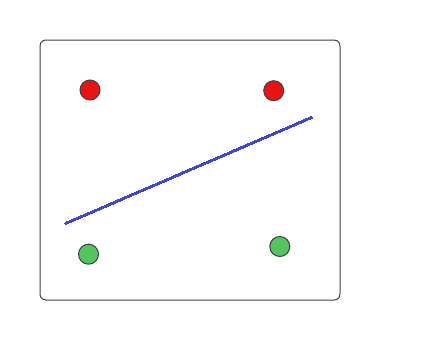
\includegraphics{images/Dichotomy 1.png}
    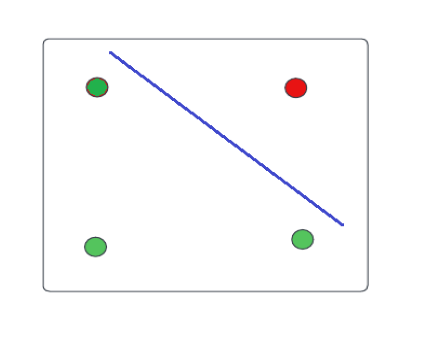
\includegraphics{images/Dichotomy 2.png}
\end{center}
Let's consider a plane with 4 points. If we choose the hyperplanes in $\mathbb{R}^{2}$ as hypothesis space $H$ we can divide the points with a line and classify them with two colors (red and green). These partitions are called dichotomies. Note that this particular $H$ \textbf{can't} implement all possible dichotomies.
\begin{figure}[h]
    \centering
    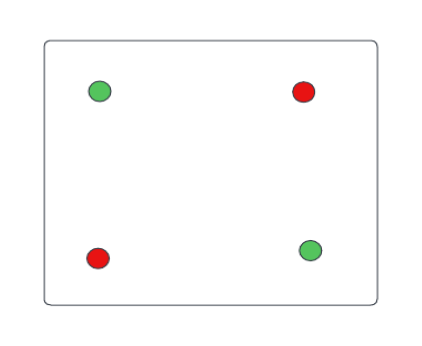
\includegraphics{images/Dichotomy 3.png}
    \caption{This classification can't be implemented by any hyperplane in $H$}
\end{figure} \newline
\begin{itemize}
    \item \textbf{Shattering: } Given $S \subset X, S$ is shattered by the hypothesis space $H$ iff 
    \[\forall S^{'} \subseteq S, \exists h \in H, s.t. \forall x \in S, h(x) = 1 \iff x \in S^{'}\]
    That means that $H$ is able to implement all possible dichotomies of $S$.
    
    \item \textbf{VC-dimension: } The VC-dimension of an hypothesis space $H$ defined over an instance space $X$ is the size of the largest finite subset of $X$ shattered by $H$: 
    \[VC(H) = \max_{S \subseteq X}|S|\]
    such that S is shattered by $H$.
\end{itemize}

If we consider $H_{1} = \{f_{w,b}(y) | f_{w,b}(y) = sign(w \cdot y + b), w \in \mathbb{R}^{2}, b \in \mathbb{R}\}$ as hypothesis space (hyperplanes in $\mathbb{R}^{2}$), as we saw before $VC(H_{1}) = 3$ because it doesn't exist \textbf{any} configuration of 4 points that can be shattered by $H_{1}$. In general, VC-dimension of hyperplanes in $\mathbb{R}^{n} = n + 1$: in 2 dimensions $VC(H) = 3$, in 3 dimensions $VC(H) = 4$ and so on.

\subsection{VC bound and SRM}
Consider a binary classification learning problem with:
\begin{itemize}
    \item Training set $S = \{(\textbf{x}_{1},y_{1}),...,(\textbf{x}_{n},y_{n})\}$.
    \item Hypothesis space $H = \{h_{\theta}(\textbf{x})\}$.
    \item Learning algorithm $L$, returning the hypothesis $g = h_{\theta}^{*}$ minimizing the empirical error on $S$, that is $g = argmin_{h \in H}error_{S}(h)$.
\end{itemize}
It is possible to derive \footnote{We will not see the derivation here.} an upper bound of the ideal error which is valid with probability $(1-\delta)$, $\delta$ being arbitrarily small, of the form:
\[error(g) \leq error_{S}(g) + F(\frac{VC(H)}{n},\sigma)\]
where $error(g)$ is the ideal error. The term $F(\frac{VC(H)}{n},\sigma)$ is called \textbf{VC-confidence} and it depends on:
\begin{itemize}
    \item The training size $n$ (inversely).
    \item The VC-dimension of $H VC(H)$ (proportionally).
    \item The confidence $\sigma$ (inversely).
\end{itemize}
As the VC-dimension grows, you usually observe that the empirical error decreases and that the VC confidence increases. So you can use the inductive principle \textbf{Structural Risk Minimization (SRM)} in order to minimize the right side of the confidence bound to get a tradeoff between the empirical error and the VC confidence.
\begin{figure}[h]
    \centering
    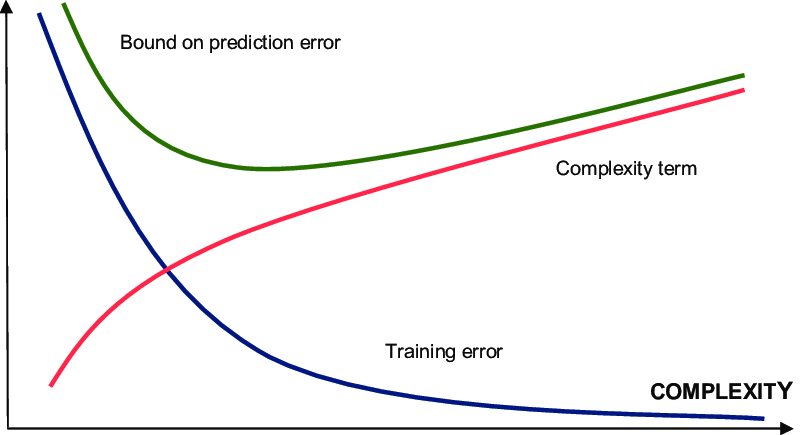
\includegraphics[scale=0.3]{images/Structural-risk-minimization-principle-Vapnik-1998.png}
    \caption{The green curve \textit{Bound on prediction error} is the sum between empirical error curve and VC confidence curve.}
\end{figure}
